\documentclass[12pt,a4paper]{article}
\usepackage[margin=2cm]{geometry}
\usepackage[utf8]{inputenc}
\usepackage[T1]{fontenc}
\usepackage{newtxtext,newtxmath}
\usepackage{graphicx}
\usepackage{booktabs}
\usepackage{array}
\usepackage{longtable}
\usepackage{caption}
\usepackage{amsmath}
\usepackage{enumitem}
\usepackage[colorlinks=false,pdfborder={0 0 0}]{hyperref}
\usepackage{titlesec}
\usepackage{fancyhdr}
\usepackage{setspace}
\usepackage{tikz}
\usepackage{ragged2e}
\usetikzlibrary{arrows.meta,positioning,shapes.geometric}

% ---- Black and white only. No colour used anywhere in this document. ----

\titleformat{\section}{\normalfont\large\bfseries}{\thesection.}{0.6em}{}
\titleformat{\subsection}{\normalfont\normalsize\bfseries}{\thesubsection}{0.6em}{}
\titleformat{name=\subsection,numberless}{\normalfont\small\bfseries}{}{0em}{}

\pagestyle{fancy}
\fancyhf{}
\setlength{\headheight}{14.5pt}
\fancyhead[L]{\footnotesize Compound Climate Disruption DSS}
\fancyhead[R]{\footnotesize UbuntuNet Alliance -- AI for Climate Resilience}
\fancyfoot[C]{\thepage}
\renewcommand{\headrulewidth}{0.4pt}
\renewcommand{\footrulewidth}{0pt}

\setstretch{1.15}
\setlength{\parindent}{0pt}
\setlength{\parskip}{6pt}

\newcommand{\sectionlimit}[1]{\textit{\small (Section limit: #1)}\par\vspace{2pt}}

\begin{document}

% ============================================================
% COVER PAGE
% ============================================================
\begin{titlepage}
\centering
\vspace*{0.4cm}

\IfFileExists{SU-LOGO.png}{
  \makebox[\linewidth]{
    \begin{tikzpicture}
      \node[minimum width=2.6cm, minimum height=2.6cm, align=center, inner sep=0pt]
        {\includegraphics[width=2.6cm, height=2.6cm, keepaspectratio]{SU-LOGO.png}};
    \end{tikzpicture}
  }
}{
  \makebox[\linewidth]{
    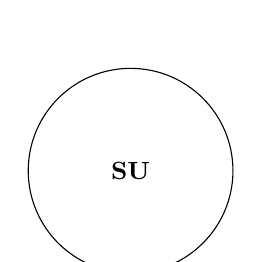
\begin{tikzpicture}
      \node[draw, circle, minimum width=2.6cm, minimum height=2.6cm, align=center,
            font=\small\bfseries, inner sep=0pt] {SU};
    \end{tikzpicture}
  }
}

\vspace{0.4cm}
{\large \textbf{STRATHMORE UNIVERSITY}\par}
{\normalsize iLabAfrica Research Centre\par}
\vspace{0.15cm}
{\normalsize Nairobi, Kenya\par}

\vspace{1.1cm}
{\small \textbf{UBUNTUNET ALLIANCE -- CALL FOR PROPOSALS}\par}
{\small AI for Climate Resilience in Africa\par}
{\small Co-funded by the European Union through AfricaConnect 4\par}

\vspace{1.3cm}
{\LARGE \textbf{From Prototype to Pilot:}\par}
\vspace{0.35cm}
{\Large \textbf{An AI-Enabled Compound Climate Disruption}\par}
{\Large \textbf{Decision-Support System for Kenya's 47 Counties}\par}

\vspace{0.6cm}
{\normalsize Predicting and Prioritising Household and County-Level Climate Risk\par}
{\normalsize from Water, Electricity, Road and Flooding Shocks using Machine Learning,\par}
{\normalsize Explainable AI and Data Envelopment Analysis\par}

\vspace{1.3cm}
{\normalsize \textbf{Full Proposal -- Grant Application}\par}

\vspace{1.0cm}
{\normalsize
\begin{tabular}{@{}ll@{}}
Lead Institution: & Strathmore University, iLabAfrica Research Centre \\[4pt]
Principal Investigator: & David Mauti \\[4pt]
Technical Lead: & Jakes Kariuki \\[4pt]
Climate Domain Lead: & Simion Mbumbu \\[4pt]
Data and Governance Lead: & Gracious Ngetich \\[4pt]
Partnership \& User Engagement Lead: & Isaac Baya \\[4pt]
Data Engineer: & Valerie Jerono \\[4pt]
\end{tabular}\par}

\vspace{1.1cm}
{\normalsize Requested Funding: US\$10,000 \quad|\quad Duration: 12 Months\par}

\vspace{1.1cm}
{\normalsize Submitted to the UbuntuNet Alliance for Research and Education Networking\par}
{\normalsize grants@ubuntunet.net\par}

\vspace{1.3cm}
{\normalsize August 2026\par}

\end{titlepage}

% ============================================================
% 1. PROJECT SUMMARY
% ============================================================
\section{Project Summary}
\sectionlimit{Max. 300 words}

Climate change in Kenya rarely arrives as a single shock. Households in flood-prone, poorly-served counties typically face \textbf{compound infrastructure disruption} -- water supply failure, impassable roads, electricity outages and localised flooding occurring together -- yet county governments still allocate adaptation resources using generic vulnerability maps rather than household-level evidence. Our team has already built and tested a working AI prototype that closes this gap. Using the nationally representative Kenya Housing Survey 2023/24 (21,347 households, 47 counties), we engineered a compound climate disruption target and trained an ensemble machine learning model (HistGradientBoosting) that predicts which households and counties face simultaneous climate-linked infrastructure failure, achieving a ROC-AUC of 0.881 -- a 9.8-percentage-point improvement over a non-AI logistic regression baseline. We layered on SHAP explainability to make every prediction auditable, and a Data Envelopment Analysis (DEA-BCC) model that scores each county's adaptation capacity relative to its resources. The two are fused into a population-weighted \textbf{Urgency Index} and Policy Quadrant Matrix that tells a county officer, in one number, whether their county needs emergency funding, capacity mobilisation, preventative structural investment, or is a best-practice model to replicate. A working choropleth dashboard with an AI assistant has already been built on this output. This project will take that proof-of-concept -- currently a research notebook and a static dashboard -- and turn it into a deployed, user-tested decision-support tool piloted with two County Climate and Environment Departments and Kenya's National Disaster Management Authority (NDMA). At the end of 12 months we will have a live, county-facing web application, documented user feedback from a real government pilot, and evidence-based reprioritisation of adaptation resources reaching an estimated 21.3 million Kenyans identified as being at compound climate risk by 2026.

% ============================================================
% 2. PROBLEM DEFINITION
% ============================================================
\newpage
\section{Problem Definition}
\sectionlimit{Max. 1 page}

Kenya's exposure to climate variability is well documented at the national level, but the *operational* problem facing county governments is different: climate risk in Kenya does not usually show up as one clean hazard. It shows up as \textbf{compounding infrastructure failure}. A single flood event can simultaneously cut a household off from piped water, wash out the only feeder road, and knock out the local electricity transformer -- and our analysis of the Kenya Housing Survey (KHS) 2023/24 confirms this is already the norm, not the exception: \textbf{35.5\% of the 21,347 surveyed households} report experiencing at least one of water disruption, road access failure, electricity outage, or neighbourhood flooding, and electricity disruption alone affects \textbf{31.6\%} of households nationally.

The people affected are concentrated, not evenly spread. Our county-level analysis shows that four counties -- Taita-Taveta, Kakamega, Busia and Kwale -- carry \textbf{critical urgency}, combining high predicted household risk with weak adaptation capacity, and a further thirteen counties sit at high urgency. Scaled against 2026 population projections (55.77 million citizens nationally, escalated from the 2019 KNBS census at a 2.3\% CAGR), our model estimates that \textbf{21.3 million Kenyans (38.2\% of the projected population)} live in households at elevated risk of compound climate disruption. Kakamega and Nairobi alone each carry more than 1.5 million and 3.0 million at-risk citizens respectively, illustrating that this is simultaneously a rural infrastructure problem and an urban resilience problem.

The institutional gap is not a lack of data -- Kenya already runs a national household survey and a rich administrative dataset on water, roads and electricity. The gap is that this data has never been fused into a predictive, prioritisation-ready tool that a county planner, KMD forecaster, or NDMA officer can actually use. County Integrated Development Plans and disaster response budgets are currently allocated using historical incident reports and generic exposure maps, which are reactive by design: they tell a county what has already gone wrong, not which specific wards and household clusters are statistically most likely to face compound shocks next, or which counties are under-performing relative to the adaptation resources they already have. Non-AI approaches -- simple hazard overlays or single-indicator vulnerability indices -- cannot capture the *interaction* between physical hazard exposure, structural housing fragility, road isolation and economic strain that actually predicts compound disruption; our own baseline comparison shows that a standard logistic regression model, which is the realistic non-AI alternative, underperforms our ensemble model by 9.8 points of ROC-AUC and 14.5 points of PR-AUC on the same task, on the same held-out households. Existing approaches are, in short, insufficiently granular, insufficiently explainable to non-technical county officers, and insufficiently linked to a governance-capacity measure that would let national government target scarce adaptation funding to where it is most needed and least available.

% ============================================================
% 3. EXISTING PROOF-OF-CONCEPT
% ============================================================
\newpage
\section{Existing Proof-of-Concept}
\sectionlimit{Max. 2 pages}

\subsection{What Currently Exists}
Our team has already built and executed, end-to-end, a working AI prototype -- not a plan for one. The artefact is a fully reproducible analytical pipeline (\texttt{AI\_CLIMATE\_RESILIENCE.ipynb}) plus a \textbf{live, deployed decision-support dashboard}, built on the nationally representative KHS 2023/24 microdata (21,347 households, 47 counties, 528 raw variables). The prototype spans the full analytical chain:

\begin{enumerate}[leftmargin=1.2em, itemsep=1pt]
\item \textbf{Target engineering.} \texttt{compound\_climate\_disruption} is defined as any household reporting water disruption, road access failure, electricity outage, or flooding (35.5\% national prevalence), with a strict anti-leakage rule excluding all four source columns from the feature set.
\item \textbf{A 34-feature predictive model} spanning hazard exposure, dwelling quality, utility access, demographics and county governance context, trained on a leakage-safe, stratified 70/15/15 split (14,942 / 3,202 / 3,203 households).
\item \textbf{A genuine non-AI baseline}: a class-weighted Logistic Regression, benchmarked against two AI ensembles (Random Forest, HistGradientBoosting) on the same held-out test set.
\item \textbf{Explainable AI}: SHAP attribution identifying the drivers of compound risk at population and household level.
\item \textbf{A County Climate Adaptation Capacity Index (CACI)}, via input-oriented Data Envelopment Analysis (DEA-BCC, PuLP), benchmarking each county's outcomes against its adaptation resources.
\item \textbf{An integrated Urgency Index and Policy Quadrant Matrix} fusing risk, vulnerability and capacity into one ranked, actionable output per county.
\item \textbf{A working, deployed front-end}: a live choropleth dashboard (all 47 counties, KPI panel, sortable table, and an AI assistant grounded on the model output), publicly accessible at \url{https://kenya-ai-climate-resilience.vercel.app/}.
\end{enumerate}

\subsection{Evidence That It Works}
This is not a conceptual pipeline -- it has been run on real held-out data and produces validated, reproducible metrics.

\begin{center}
\begin{tabular}{lccc}
\toprule
\textbf{Model} & \textbf{ROC-AUC} & \textbf{PR-AUC} & \textbf{Type} \\
\midrule
Logistic Regression (class-weighted) & 0.782 & 0.667 & Non-AI baseline \\
Random Forest (balanced subsample) & 0.855 & 0.765 & AI ensemble \\
\textbf{HistGradientBoosting (best model)} & \textbf{0.881} & \textbf{0.812} & AI ensemble \\
\bottomrule
\end{tabular}
\end{center}

On the 3,203-household held-out test set, the AI ensemble delivers a \textbf{+0.098 ROC-AUC and +0.145 PR-AUC} improvement over the realistic non-AI alternative -- direct, quantified evidence that AI materially improves predictive capability, as required by this call. The decision threshold was independently tuned on the validation set (0.512, F1 = 0.734) before being applied, untouched, to the test set, avoiding threshold leakage.

SHAP attribution confirms the model's drivers are physically and institutionally sensible -- electricity grid stability, road condition, dwelling exposure, and household income/dependency burden -- rather than spurious correlations, which matters directly for the transparency and auditability county officers will require before trusting the tool with resource-allocation decisions.

At the county level, the DEA-BCC model produced a full CACI ranking for all 47 counties, and the integrated Urgency Index identified \textbf{4 counties at critical urgency, 13 at high, 16 at moderate, and 14 at low}, with Taita-Taveta, Kakamega, Busia and Kwale ranking highest -- concentrating an estimated 3.1 million citizens in the four most critical counties alone. This output is already exported to a structured county-level CSV and powers the live dashboard, demonstrating the pipeline runs cleanly from raw survey microdata to a decision-ready, public interface -- the exact transition this call is designed to fund.

\subsection{Technology Readiness Level and Honest Gaps}
By the TRL scale, we assess the current prototype at \textbf{TRL 5} (validated in a relevant environment: the dashboard is deployed and publicly accessible at \url{https://kenya-ai-climate-resilience.vercel.app/}, built on an earlier iteration of the same pipeline that powers our live water-vulnerability tool, \texttt{water-futures.vercel.app}, SMOTE-LightGBM, ROC-AUC 0.92). We are honest about what remains -- precisely the gaps this grant will close:

\begin{itemize}[leftmargin=1.2em, itemsep=1pt]
\item No county government, NDMA, or WASREB representative has yet used the live tool -- target users are identified (Section 4) but a structured pilot with documented feedback has not yet run.
\item The model uses a single cross-sectional survey wave (KHS 2023/24); it does not yet ingest real-time weather/hydrological signals or have a maintained data-refresh pipeline for future survey rounds.
\item SHAP and CACI outputs exist in the dashboard but not yet as plain-language, per-county explanations tailored for a non-technical planning officer.
\end{itemize}

% ============================================================
% 4. PROPOSED TRANSITION FROM POC TO PILOT
% ============================================================
\newpage
\section{Proposed Transition from Proof-of-Concept to Pilot}
\sectionlimit{Max. 3 pages}

\subsection{AI Approach and Data Inputs}
We will carry forward the validated modelling architecture from the proof-of-concept unchanged in substance -- the 34-feature, leakage-audited HistGradientBoosting classifier (ROC-AUC 0.881), SHAP attribution layer, and DEA-BCC County Climate Adaptation Capacity Index -- and invest the grant period in three things the PoC does not yet have: a live, user-facing application; real government users; and a documented pilot. Data inputs remain the existing KHS 2023/24 microdata and county administrative indicators (water system efficiency, EIA approval rates, planning staff counts, storage capacity) already used in the PoC, meaning \textbf{no new primary data collection is required} -- a direct response to this call's preference for projects that build on datasets that already exist. Where county partners can supply updated administrative figures during the pilot (e.g. current water storage capacity or planning staff establishment), we will refresh the CACI inputs for their county specifically, giving pilot counties a more current picture than the notebook baseline.

\subsection{From Notebook to Application}
The transition path is deliberately narrow and de-risked, because our team has already executed this exact transition once before, on the related Water Futures prototype, which is live in production today. Concretely, we will:

\begin{enumerate}[leftmargin=1.2em]
\item \textbf{Harden and deploy the existing dashboard.} The static dashboard build already in hand (choropleth map, KPI panel, sortable 47-county table, and a natural-language assistant grounded on the model's own output) will be deployed to a public URL, then extended into a \textbf{county-planner workflow view}: a per-county drill-down page showing the county's Urgency tier, Policy Quadrant classification, recommended intervention, SHAP-based plain-language risk drivers, and CACI peer-benchmarking against comparable counties.
\item \textbf{Add a role-appropriate explanation layer.} We will translate SHAP outputs (currently a technical beeswarm plot) into short, plain-language "why this county is flagged" summaries, so that a Climate and Environment Officer without a data science background can trust and act on the score without needing to interpret a model artefact directly -- directly addressing the UNESCO transparency requirement in Table 1 of the call.
\item \textbf{Refresh and validate with pilot-county data.} We will engage two pilot counties selected from our current Critical/High urgency ranking (prioritising a rural county such as Kakamega or Busia and an urban county such as Nairobi or Mombasa, to test the tool across contrasting operating environments), incorporate any updated administrative figures they can share, and re-run the CACI and Urgency computation for those counties as a validation exercise.
\item \textbf{Run a bounded micro-pilot.} Over a defined testing window, County Climate and Environment Department staff and an NDMA liaison will use the dashboard to review current risk rankings against their own institutional knowledge, flag discrepancies, and complete a structured usability and trust survey, generating the credible evidence of usability and value this call explicitly asks for.
\item \textbf{Iterate on the interface and, where warranted, the model,} based on pilot feedback -- for example, adding filters county officers request, or recalibrating thresholds if pilot users identify systematic false positives/negatives in their own local knowledge.
\item \textbf{Document and disseminate}, producing a short technical validation note and a public case-study brief usable for follow-on funding conversations with WASREB, NDMA, or county governments beyond the two pilot sites.
\end{enumerate}

\subsection{Innovation: Technical, Contextual and Practical}
The technical novelty of this project is not any single algorithm -- it is the \textbf{fusion of three distinct analytical layers into one decision} that a county officer can act on immediately: (i) a predictive layer (who is at risk, and why, via ML + SHAP); (ii) a governance-efficiency layer (which counties are underperforming relative to their own resources, via DEA-BCC); and (iii) a population-weighted prioritisation layer that combines both into a single, ranked, four-quadrant policy recommendation. To our knowledge, no existing Kenyan climate dashboard combines a validated compound-shock risk model with a formal efficiency-frontier governance benchmark in a single, county-facing tool. Contextual relevance comes from grounding every input in Kenya's own national household survey and administrative data, rather than global climate-exposure proxies that do not reflect local infrastructure realities. Practical applicability comes from the explicit design decision to require no real-time satellite feeds or IoT sensor networks -- the tool works today, in data-constrained county offices, on data Kenya already collects.

\subsection{Expected System Maturity After Project Completion}
We expect the system to reach \textbf{TRL 6/7} by month 12: a technology demonstrated in a relevant, real operational environment (two county government pilots), with documented user feedback, rather than a laboratory-only artefact. Concretely, tangible and measurable outputs are:

\begin{itemize}[leftmargin=1.2em]
\item A publicly accessible, live decision-support web application covering all 47 counties.
\item A documented pilot in at least two county government departments, with a structured usability/trust evaluation (target: at least 10 individual users across the two pilot sites, and a usability score benchmark established for future scale-up conversations).
\item A plain-language, SHAP-derived explanation layer embedded directly in the interface for every county.
\item A refreshed, validated CACI and Urgency ranking for the two pilot counties incorporating current administrative data.
\item A public technical brief and case-study document suitable for follow-on funding applications (e.g. to WASREB, NDMA, or national climate finance mechanisms) and for submission as a peer-reviewed conference or working paper output from Strathmore University.
\end{itemize}

We are also explicit about the impact we are \textit{not} claiming: this grant funds a bounded, two-county micro-pilot, not a national rollout, and it does not fund new primary data collection or continuous real-time monitoring. Those are natural, well-evidenced next stages that a successful pilot -- with the credible usage evidence this call is designed to generate -- would put us in a strong position to pursue with larger funders.

% ============================================================
% 5. IMPLEMENTATION PLAN AND TIMELINE
% ============================================================
\newpage
\section{Implementation Plan and Timeline}
\sectionlimit{Max. 1 page}

\begin{center}
\begin{tabular}{@{}p{2.0cm}p{7.6cm}p{5.8cm}@{}}
\toprule
\textbf{Phase} & \textbf{Key Activities} & \textbf{Milestone / Responsible} \\
\midrule
Months 1--3 &
Harden existing dashboard for public deployment; build county drill-down and plain-language SHAP explanation views; identify and formally engage two pilot counties and an NDMA liaison; secure letters of collaboration. &
Live dashboard deployed; two signed pilot-county engagements. \newline \textit{Technical Lead; Partnership \& User Engagement Lead} \\
\addlinespace
Months 4--6 &
Refresh CACI/Urgency inputs with pilot-county administrative data; onboard pilot users; run structured micro-pilot sessions and usability/trust survey; log discrepancies against local institutional knowledge. &
Pilot sessions completed in both counties; usability data collected. \newline \textit{Principal Investigator; Climate Domain Lead} \\
\addlinespace
Months 7--9 &
Iterate on interface and model calibration based on pilot feedback; strengthen data governance documentation; begin scoping integration with NDMA early-warning workflows. &
Revised, pilot-informed version of the tool released. \newline \textit{Data and Governance Lead; Technical Lead} \\
\addlinespace
Months 10--12 &
National dissemination (all 47 counties visible on the live dashboard); publish technical validation brief and case study; prepare peer-reviewed / conference submission; compile follow-on funding package. &
Public brief published; follow-on funding proposal drafted. \newline \textit{Principal Investigator; Data Engineer} \\
\bottomrule
\end{tabular}
\end{center}

Risk buffer: each phase reserves the final two weeks for catch-up, since pilot scheduling depends on county government availability outside our control (mitigation detailed in Section 8).

% ============================================================
% 6. PROJECT TEAM AND ROLES
% ============================================================
\newpage
\section{Project Team and Roles}
\sectionlimit{Max. 2 pages}

Our team is deliberately structured to cover the full chain this call requires: technical AI delivery, climate-domain grounding, data governance, and real user/partner engagement -- and we already have a track record of shipping a related tool together.

\begin{center}
\small
\begin{tabular}{@{}p{2.3cm}p{2.7cm}p{9.3cm}@{}}
\toprule
\textbf{Name} & \textbf{Role} & \textbf{Contribution to This Project} \\
\midrule
David Mauti & Principal Investigator &
Overall accountability, coordination across delivery phases, and primary liaison with Strathmore University and UbuntuNet Alliance on compliance and reporting. Co-developed the earlier Water Futures prototype with Jerono and Ngetich -- direct prior experience taking a similar model from notebook to live tool. \\
\addlinespace
Jakes Kariuki & Technical Lead &
Owns the technical transition to deployed application: hardening the dashboard, extending the SHAP explanation layer, and integrating pilot-county data refreshes into the pipeline. \\
\addlinespace
Simion Mbumbu & Climate Domain Lead &
Grounds the project in Kenya's climate adaptation policy landscape; validates that risk drivers and recommended interventions are institutionally realistic; leads engagement content for county officers and NDMA. \\
\addlinespace
Gracious Ngetich & Data and Governance Lead &
Owns data quality, privacy and responsible-AI documentation; oversees the anti-leakage/provenance discipline already built into the PoC. Co-founder (engineering), Vondetta, an AI and decision-intelligence firm serving African insurers -- production data-governance experience. \\
\addlinespace
Isaac Baya & Partnership \& User Engagement Lead &
Formally engages the two pilot counties and the NDMA liaison; secures letters of collaboration; designs and runs the structured usability/trust survey. \\
\addlinespace
Valerie Jerono & Data Engineer &
Maintains the KHS 2023/24 pipeline (extraction, cleaning, feature engineering, anti-leakage audit); supports CACI/DEA-BCC computation and county data refresh. MSc Data Science candidate, Strathmore iLabAfrica; founder, Vondetta. \\
\bottomrule
\end{tabular}
\end{center}

\subsection{Prior Collaboration and Readiness}
Three of six members (Mauti, Ngetich, Jerono) already delivered a directly related tool together -- a household water-vulnerability prototype on the same survey data and methodology, deployed live and submitted to the Strathmore Ideas Festival 2026 -- so this team is repeating, not learning, a notebook-to-production path. Formal CVs, publication records and partner letters of support are being finalised alongside submission and appended where available (Appendix A/B); any outstanding item will reach the Alliance before the announcement date, and the PI and Partnership Lead jointly cover any interim gap in Months 1--3.

% ============================================================
% 7. DATA AND INFRASTRUCTURE
% ============================================================
\newpage
\section{Data and Infrastructure}
\sectionlimit{Max. 1 page}

\textbf{Data sources.} The core dataset is the Kenya Housing Survey 2023/24 (KHS), a nationally representative household survey administered by the Kenya National Bureau of Statistics (KNBS), which our team already holds and has processed (21,347 households, 47 counties). County-level administrative indicators used in the CACI model (EIA approval rates, water system efficiency, planning staff counts, water storage capacity) are drawn from existing public/administrative sources already integrated into the proof-of-concept. Population projections use the 2019 KNBS Census escalated to 2026 at a 2.3\% CAGR. \textbf{No new primary household data collection is required for this project} -- pilot counties will be asked only to confirm or update a small number of already-modelled administrative indicators specific to their county.

\textbf{Access arrangements.} The KHS 2023/24 microdata is already in our possession under existing academic access arrangements through Strathmore University; no new data-sharing agreement is required to continue using it. Any county-specific administrative data shared during the pilot will be provided directly by pilot-county officers under a data-sharing understanding documented in the letters of collaboration.

\textbf{Data governance.} All modelling work follows the anti-leakage and stratified-validation discipline already built into the proof-of-concept (target-defining columns strictly excluded from features; all preprocessing fitted on training data only). The Data and Governance Lead will maintain a data dictionary and provenance log for any pilot-county data ingested, and will document known limitations of the KHS sampling frame (e.g. potential under-representation of the most remote, hardest-to-reach households, who may in fact be at the highest compound-disruption risk) transparently in both the technical brief and the user-facing dashboard.

\textbf{Technical infrastructure.} The application layer is intentionally lightweight and low-cost, consistent with this call's preference against large infrastructure spend: a static front-end (HTML/JS, choropleth mapping) served from a standard cloud hosting platform, a small serverless function for the natural-language assistant, and no dedicated database or GPU infrastructure required. The modelling pipeline runs on standard Python data-science tooling (pandas, scikit-learn, SHAP, PuLP) and can be re-executed on any standard cloud or university compute resource. \textbf{Dependency on external systems} is limited to: (i) a third-party large-language-model API for the optional natural-language assistant feature (non-critical -- the core map, KPI and table views function fully without it), and (ii) standard cloud hosting for the static site and serverless function. Both are low-cost, replaceable, and do not create lock-in risk to the core decision-support functionality.

% ============================================================
% 8. GOVERNANCE, ETHICS AND RISK MANAGEMENT
% ============================================================
\newpage
\section{Governance, Ethics and Risk Management}
\sectionlimit{Max. 1.5 pages}

\subsection{Risk Register}
\begin{center}
\small
\begin{tabular}{@{}p{2.1cm}p{6.4cm}p{6.0cm}@{}}
\toprule
\textbf{Risk} & \textbf{Description} & \textbf{Mitigation} \\
\midrule
Technical / model &
Model or SHAP outputs do not generalise well to a specific pilot county's local context. &
Re-validate against county officer knowledge at onboarding; treat disagreement as iteration data, not failure; limitations documented in-interface. \\
\addlinespace
Data quality/access &
County-supplied administrative data during the pilot is incomplete, delayed or inconsistent with KHS baselines. &
Pilot proceeds on the validated KHS baseline regardless; county data is an enhancement, not a dependency; provenance log flags source of every figure. \\
\addlinespace
Operational / adoption &
Officer time and institutional coordination constraints slow engagement or usage during testing. &
Written collaboration secured before Month 1; sessions scheduled around officers' calendars; two-week buffer built into every phase. \\
\addlinespace
Deployment &
Reliance on a third-party LLM API for the assistant feature introduces cost/availability risk. &
Core dashboard (map, KPIs, table) works fully without the assistant; it is scoped as an enhancement on a low/no-cost tier. \\
\bottomrule
\end{tabular}
\end{center}

\subsection{Alignment with Governing Frameworks}
\begin{center}
\small
\begin{tabular}{@{}p{2.9cm}p{11.6cm}@{}}
\toprule
\textbf{Framework} & \textbf{How this project aligns} \\
\midrule
AU Continental AI Strategy &
African-led and university-based, built entirely on Kenyan national data and county governance structures rather than imported proxies; strengthens a local research ecosystem (Strathmore iLabAfrica), builds a reusable local data asset (the KHS-derived county risk dataset), and is delivered by an interdisciplinary team. \\
\addlinespace
UNESCO Ethics Recommendation &
Human-centred design via a plain-language SHAP layer for non-technical officers; inclusiveness through documented KHS sampling limitations (Sec.~7) and deliberate inclusion of under-resourced counties (e.g. Taita-Taveta, Busia, Kwale) in pilot selection; data responsibility via the anti-leakage, train-only-fitting discipline already in the pipeline; transparency via a technical brief documenting assumptions and limitations. \\
\addlinespace
EU AI Act &
Classified as \textbf{decision-support}, not automated decision-making -- the tool informs a human officer and does not autonomously allocate funding. We maintain basic technical documentation (model card, data dictionary, limitations note) and pair every score with its explanation, anticipating future transparency and human-oversight requirements without claiming full regulatory compliance. \\
\bottomrule
\end{tabular}
\end{center}

\textbf{Key ethical commitment.} Because this tool ranks counties -- and, implicitly, communities -- by risk and adaptation capacity, we commit to never showing an Urgency score or CACI ranking without its explanation, and to caveating that the DEA-BCC ``efficiency frontier'' measures performance relative to existing resources, not absolute need, so a low-capacity county is read as under-resourced, not underperforming.

% ============================================================
% 9. COMMUNICATION
% ============================================================
\newpage
\section{Communication}
\sectionlimit{Max. 0.5 page}

Results will be communicated through three channels aimed at three audiences. For \textbf{pilot-county officers and NDMA}, we will hold in-person or virtual walkthroughs of the live dashboard at pilot onboarding and again at Month 9, plus a one-page, plain-language county brief generated directly from the tool. For the \textbf{national policy and research community} (WASREB, Ministry of Environment, other county governments, and the UbuntuNet Alliance), we will publish a public technical brief and case-study at project close, present findings at the UbuntuNet Connect 2027 Conference showcase, and pursue a peer-reviewed or working-paper submission through Strathmore University. For \textbf{broader uptake}, the live dashboard itself remains publicly accessible after the grant period, and our team will use documented pilot evidence to approach follow-on funders (national climate finance mechanisms, WASREB, or philanthropic partners) for scale-up beyond the two pilot counties.

% ============================================================
% 10. BUDGET AND JUSTIFICATION
% ============================================================
\newpage
\section{Budget and Justification}
\sectionlimit{Max. 2 pages}

\begin{center}
\small
\begin{tabular}{@{}p{0.5cm}p{5.4cm}p{1.3cm}p{1.9cm}p{2.0cm}p{2.0cm}@{}}
\toprule
\textbf{No.} & \textbf{Description} & \textbf{Number} & \textbf{Units} & \textbf{Unit Cost (US\$)} & \textbf{Total (US\$)} \\
\midrule
\multicolumn{6}{@{}l}{\textit{Personnel Costs}} \\
1 & Research assistant -- data validation, pilot-county data refresh and provenance logging & 1 & 12 months (part-time) & 166.67 & 2,000 \\
2 & Technical development stipend -- dashboard hardening, SHAP explanation layer, integration (Technical Lead) & 1 & 6 months (part-time) & 333.33 & 2,000 \\
\multicolumn{4}{@{}r}{\textbf{Sub-Total Personnel Costs}} & & \textbf{4,000} \\
\addlinespace
\multicolumn{6}{@{}l}{\textit{Other Costs}} \\
3 & Cloud hosting, serverless functions and LLM API costs (12 months) & 12 & months & 41.67 & 500 \\
4 & Data pipeline and compute (validation runs, pilot-county recomputation) & 1 & lump sum & 500 & 500 \\
5 & County pilot engagement -- travel, venue and per-county coordination (2 counties) & 2 & counties & 1,000 & 2,000 \\
6 & Community dissemination and training materials (pilot workshops + final brief design/print) & 1 & lump sum & 1,500 & 1,500 \\
7 & UbuntuNet Connect 2027 showcase participation (materials/registration; travel excluded, covered separately by lead institution where applicable) & 1 & lump sum & 500 & 500 \\
8 & Contingency (schedule/data-access risk buffer, Section 8) & 1 & lump sum & 1,000 & 1,000 \\
\multicolumn{4}{@{}r}{\textbf{Sub-Total Other Costs}} & & \textbf{6,000} \\
\midrule
\multicolumn{5}{@{}r}{\textbf{TOTAL BUDGET}} & \textbf{10,000} \\
\bottomrule
\end{tabular}
\end{center}

\textbf{Budget Notes.} No institutional overheads are included, in line with call requirements. Line 1 funds a research assistant to carry out the data validation, county-data ingestion, and provenance logging described in Sections 4 and 7 -- this is the single largest determinant of pilot credibility and is prioritised accordingly. Line 2 is a modest development stipend, not a full salary, reflecting that the core model and dashboard already exist and this grant funds their hardening and extension, not construction from scratch. Line 3 keeps recurring infrastructure costs to a minimum, consistent with our lightweight, no-database architecture (Section 7); the LLM-assistant feature is scoped to fit within this line using a free/low-cost provider tier, and the core decision-support functionality does not depend on it. Line 5 is sized for two counties, matching our bounded micro-pilot design (Section 4) rather than a national rollout. Line 8 provides a contingency directly tied to the two risks flagged in Section 8 (county officer scheduling delays; data-access variability) rather than being an undifferentiated buffer. We consider this budget proportionate: it funds the specific, named activities that take an already-working prototype to a documented, user-tested pilot, and nothing beyond that scope.

% ============================================================
% APPENDIX A: CVs
% ============================================================
\newpage
\section*{Appendix A: Curricula Vitae of Key Team Members}
\addcontentsline{toc}{section}{Appendix A: Curricula Vitae of Key Team Members}
\textit{Prepared using the CV template in Appendix B of the Call for Proposals. Fields marked \texttt{[TO CONFIRM]} should be completed/verified by the named individual before final submission.}

\subsection*{David Mauti -- Principal Investigator}
\textbf{Institution:} Strathmore University (SIMS School) \quad \textbf{Country:} Kenya \\
\textbf{Proposed role:} Overall project leadership, coordination, and UbuntuNet Alliance liaison; grant compliance and reporting. \\
\textbf{Relevant expertise:} Co-developer of the Water Futures household water-vulnerability prototype (deployed live, SMOTE-LightGBM model, ROC-AUC 0.92), demonstrating direct prior experience delivering a related AI decision-support tool from notebook to production. \textbf{[TO CONFIRM: core technical skills, domain expertise, degree(s) and year(s), additional relevant experience/outputs.]}

\subsection*{Jakes Kariuki -- Technical Lead}
\textbf{Institution:} \textbf{[TO CONFIRM]} \quad \textbf{Country:} Kenya \\
\textbf{Proposed role:} Technical delivery of the dashboard hardening, SHAP explanation layer, and pilot-data integration described in Section 4. \\
\textbf{Relevant expertise:} \textbf{[TO CONFIRM: core technical skills (e.g. ML, software engineering, dashboard/web development), deployment experience, degree(s), selected relevant projects and outputs.]}

\subsection*{Simion Mbumbu -- Climate Domain Lead}
\textbf{Institution:} \textbf{[TO CONFIRM]} \quad \textbf{Country:} Kenya \\
\textbf{Proposed role:} Climate and policy grounding; validation of model features and recommended interventions; engagement content for county and NDMA users. \\
\textbf{Relevant expertise:} \textbf{[TO CONFIRM: climate/environmental domain background, relevant coursework, research or field experience, degree(s), selected relevant outputs.]}

\subsection*{Gracious Ngetich -- Data and Governance Lead}
\textbf{Institution:} Strathmore University (SIMS School) \quad \textbf{Country:} Kenya \\
\textbf{Proposed role:} Data quality, privacy and responsible-AI documentation for the pilot; anti-leakage and provenance discipline oversight. \\
\textbf{Relevant expertise:} Co-founder (Engineering) of Vondetta, an AI and decision-intelligence firm serving African insurers and financial institutions; co-developer of the Water Futures water-vulnerability prototype. \textbf{[TO CONFIRM: core technical skills, degree(s) and year(s), additional relevant experience/outputs.]}

\subsection*{Isaac Baya -- Partnership \& User Engagement Lead}
\textbf{Institution:} \textbf{[TO CONFIRM]} \quad \textbf{Country:} Kenya \\
\textbf{Proposed role:} Pilot-county and NDMA engagement, letters of collaboration, and designing and administering the usability and trust survey. \\
\textbf{Relevant expertise:} \textbf{[TO CONFIRM: partnership and stakeholder engagement experience, relevant sector background, degree(s), selected relevant outputs.]}

\subsection*{Valerie Jerono -- Data Engineer}
\textbf{Institution:} Strathmore University, iLabAfrica Research Centre \quad \textbf{Country:} Kenya \\
\textbf{Email:} valerie.jerono@strathmore.edu \quad \textbf{Phone:} 0791 987 818 \\
\textbf{Proposed role:} Maintains the KHS 2023/24 data pipeline (extraction, cleaning, feature engineering, anti-leakage audit); supports CACI/DEA-BCC computation and pilot-county data refresh. \\
\textbf{Relevant expertise:} MSc Data Science and Analytics candidate, Strathmore University iLabAfrica Research Centre (May 2025 -- June 2027); BSc Actuarial Science, Daystar University (Aug 2019 -- Nov 2023); Founder, Vondetta -- an AI and decision-intelligence firm targeting African insurers and financial institutions; co-developer of the Water Futures water-vulnerability prototype. \\
\textbf{Links:} linkedin.com/in/valerie-jerono \quad github.com/VAL-Jerono

% ============================================================
% APPENDIX B: SUPPORTING MATERIALS
% ============================================================
\newpage
\section*{Appendix B: Supporting Materials}
\addcontentsline{toc}{section}{Appendix B: Supporting Materials}

\textbf{Letters of support/collaboration.} At least one letter of support or collaboration from an intended user group or institutional partner (e.g. a pilot County Climate and Environment Department, or NDMA) is required by this call and should be attached here once secured by the Partnership \& User Engagement Lead. \textbf{[TO ATTACH before final submission.]}

\textbf{Proof-of-concept evidence.} The following supporting evidence is available and should be attached or linked in the final submission package: (i) the executed analytical notebook (\texttt{AI\_CLIMATE\_RESILIENCE.ipynb}) showing all computed metrics reported in Section 3; (ii) the exported 47-county results file (\texttt{county\_climate\_recommendations.csv}); (iii) the packaged dashboard build, ready for one-step deployment; and (iv) the earlier, live Water Futures prototype (\href{https://water-futures.vercel.app/}{water-futures.vercel.app}) as evidence of this team's prior successful notebook-to-production delivery. \textbf{We recommend deploying the AI\_CLIMATE\_RESILIENCE dashboard to a public URL before final submission, so this proposal can cite a live link alongside the notebook evidence.}

\end{document}